\chapter{Umsetzung}

\section{Variantenvergleich}

\subsection{Bestehende Parallelisierungsstrategien und ihre Grenzen}

Von den in Abschnitt~\ref{ssec:par} genannten Ansätzen in der Literatur sind aufgrund ihrer Umsetzung für \gls{gpu}s die
Strategien von Xu et al.~\cite{xumuell}, Scherl et al.~\cite{scherlkeck} und Zhao et al.~\cite{zhao} von besonderem
Interesse für diese Arbeit.

Da Xu et al. 2004 mit ihrer Arbeit~\cite{xumuell} Neuland betraten, standen ihnen viele Methoden und Technologien, die
seitdem entwickelt wurden, noch nicht zur Verfügung. Die 2004 erschienenen \gls{gpu}s hatten im Vergleich zu heutigen
Grafikkarten sehr viel weniger Speicher; das damals beste verfügbare Produkt von NVIDIA{\textregistered}, die
GeForce{\textregistered} 6800 Ultra, konnte lediglich mit 512 MiB Speicher aufwarten und war nur über \gls{opengl} oder
\gls{directx} indirekt programmierbar~\cite{geforce6800}. Den begrenzten Speicher versuchte die Gruppe durch eine
Aufteilung des Volumens und eine schichtweise Rekonstruktion desselben unter Einbeziehung aller Projektionen möglichst
effizient zu nutzen. Aufgrund des technischen Fortschritts stehen uns heute andere Möglichkeiten zur Lösung dieses
Problems offen; so bietet etwa die NVIDIA{\textregistered} GeForce{\textregistered} GTX 1080 mit 8 GiB Speicher und der
Möglichkeit der direkten Programmierung mittels \gls{cuda} oder \gls{opencl} ganz andere Nutzungs- und
Berechnungsmöglichkeiten als ihre frühen Vorgänger~\cite{gtx1080}. Insbesondere ist es möglich, das ganze Volumen oder
Teile davon während der Berechnung im Speicher zu halten und dadurch häufige Kopien zwischen \gls{cpu}-Speicher und
\gls{gpu}-Speicher zu vermeiden.

Die Forschungsgruppe um Scherl~\cite{scherlkeck} baute auf der Idee, das Volumen im Speicher zu halten, auf und ging
stattdessen den Weg, jede Projektion einzeln in dieses Volumen zu projizieren. Zur Trennung bzw.\ Kapselung der
einzelnen Schritte entwickelten sie in einem vorherigen Schritt~\cite{scherlhopp} eine Pipeline-Struktur (nach Mattson
et al.~\cite{mattsan}). Jeder Schritt des \gls{fdk} wird dabei in einer eigenen Stufe (\textit{stage}) ausgeführt, die
in einem separaten Thread ausgeführt wird. Zur Kommunikation der Ergebnisse der einzelnen Stufen werden thread-sichere
Puffer verwendet, auf die die Eingabe- bzw.\ Ausgaberoutinen der Stufen zugreifen.

Die Grenzen bei dem vorgeschlagenen Verfahren der Gruppe um Zhao et al.~\cite{zhao} sind vor allem praktischer Natur.
Das von ihnen vorgestellte Modell sieht vor, Symmetrien auszunutzen und dadurch Rechenzeit einzusparen. Sie machen sich
dabei den Umstand zunutze, dass die auf den Detektor projizierte Koordinate eines \gls{voxel}s der um 90° rotierten
Projektionskoordinate des um den gleichen Betrag rotierten Voxels entspricht. Auf diese Weise lassen sich durch eine
Berechnung die Detektorkoordinaten von vier \gls{voxel}n finden, was eine Verkürzung der Rechenzeit verspricht. In der
Praxis scheitert dieses Verfahren an dem mechanischen Aufbau üblicher CT-Scanner. Da entweder Quelle und Detektor oder
aber das Untersuchungsobjekt rotiert werden müssen, kommt es durch Fehler in der Mechanik häufig dazu, dass Aufnahmen
doppelt gemacht oder übersprungen werden; auch kann es passieren, dass die Winkelschritte zwischen zwei Aufnahmen nicht
immer einheitlich sind.

\subsection{Das Problem des GPU-Speichers}

\subsection{Heterogene GPU-Systeme und effiziente Arbeitsteilung}

\section{Implementierung und Optimierung}

In diesem Abschnitt werden die Implementierung und die Optimierung des \gls{fdk} beschrieben. Zunächst werden die
Implementierungs- und Optimierungsziele sowie die Einflüsse der realen Welt auf das Modell vorgestellt und im Anschluss
daran die Umsetzung der Stufen \textit{Wichtung} und \textit{Filterung} gezeigt. Der Abschnitt schließt mit der
Implementierung der Rückprojektion.

\subsection{Implementierungs- und Optimierungsziele}

\begin{itemize}
    \item Wartbarkeit
    \item Portabilität
    \item sinnvolle Geschwindigkeit
    \item nutzbar auf Laptop / Workstation / GPU-Cluster
\end{itemize}

\subsection{Einflüsse der realen Welt}

Die in Kapitel~\ref{chap:grundlagen} gezeigten Überlegungen zur gefilterten Rückprojektion und dem \gls{fdk} sind in
dieser Form rein theoretischer Natur. Die Anwendung dieser Modelle auf die reale Welt ist mit einigen Schwierigkeiten
bzw.\ Einflüssen verbunden, die im Folgenden näher vorgestellt werden sollen.

\subsubsection{Detektorgeometrie}

Der Detektor übt aufgrund der durch ihn gewonnenen Informationen (in Form der Projektionen) einen großen Einfluss auf
die gefilterte Rückprojektion aus. Seinem Aufbau muss daher bei der Implementierung des \gls{fdk} besondere
Aufmerksamkeit zukommen.

Der Detektor hat eine feste Breite und Höhe (gemessen in Millimetern) und besteht aus einer zweidimensionalen Anordnung
von \gls{pixel}n (siehe Abbildung~\ref{fig:det_geometrie}). In der horizontalen Richtung verfügt er über $N_h$
\gls{pixel}, in der vertikalen Richtung sind es $N_v$ \gls{pixel}.

Jedes \gls{pixel} hat eine physische Breite $d_h$ und Höhe $d_v$ (gemessen in Millimetern); äquivalent lassen sich diese
Ausdehnungen als horizontale (vertikale) Abstände zwischen den \gls{pixel}zentren betrachten (siehe
Abbildung~\ref{fig:det_pixel}).

Spannt man nun über dem Detektor ein Koordinatensystem auf (mit dessen Zentrum als Ursprung, siehe
Abbildung~\ref{fig:det_koord}), wobei $h_{min}$, $h_{max}$, $v_{min}$ und $v_{max}$ den horizontalen (vertikalen)
Abstand von den Detektorrändern bis zur Detektormitte in Millimetern angeben, so ergeben sich die folgenden
Zusammenhänge:

\begin{equation}\label{eq:det_h}
    \begin{aligned}
        h_{max} - h_{min} &= N_h \cdot d_h\\
        h_{min} + \frac{N_h \cdot d_h}{2} &= 0
    \end{aligned}
\end{equation}

\begin{equation}\label{eq:det_v}
    \begin{aligned}
        v_{max} - v_{min} &= N_v \cdot d_v\\
        v_{min} + \frac{N_v \cdot d_v}{2} &= 0
    \end{aligned}
\end{equation}

\begin{figure}[!tb]
    \centering
    \begin{minipage}[b]{.5\textwidth}
        \centering
        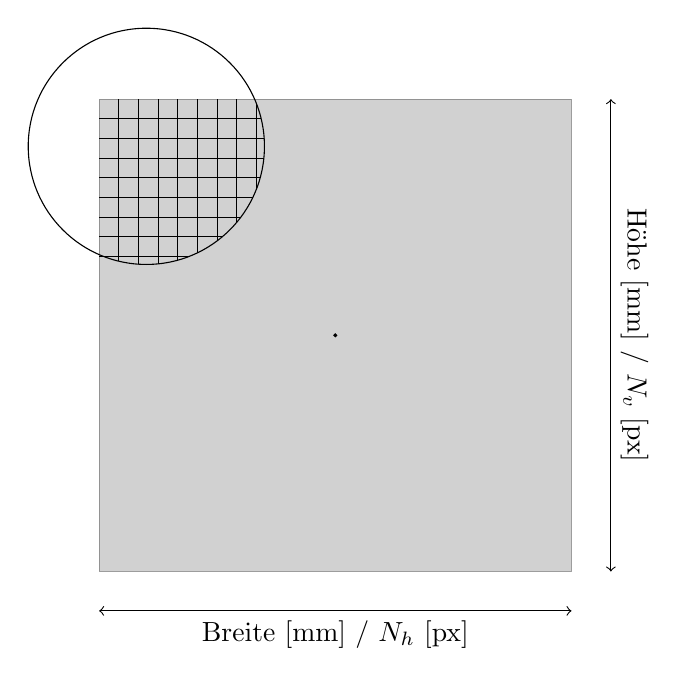
\begin{tikzpicture}
            \draw[fill=black!60!white,opacity=0.3] (-3, 3) -- (3, 3) -- (3, -3) -- (-3, -3) -- (-3, 3);
            \draw[fill=black] (0,0) circle (0.5pt);

            % Lupe
            \draw (-2.4, 2.4) circle (1.5cm);

            % Pixellinien vertikal
            \draw (-2.75, 3) -- (-2.75, 0.95);
            \draw (-2.5, 3) -- (-2.5, 0.9);
            \draw (-2.25, 3) -- (-2.25, 0.9);
            \draw (-2, 3) -- (-2, 0.95);
            \draw (-1.75, 3) -- (-1.75, 1.05);
            \draw (-1.5, 3) -- (-1.5, 1.2);
            \draw (-1.25, 3) -- (-1.25, 1.43);
            \draw (-1, 2.94) -- (-1, 1.85);

            % Pixellinien horizontal
            \draw (-3, 2.75) -- (-0.95, 2.75);
            \draw (-3, 2.5) -- (-0.9, 2.5);
            \draw (-3, 2.25) -- (-0.9, 2.25);
            \draw (-3, 2) -- (-0.95, 2);
            \draw (-3, 1.75) -- (-1.05, 1.75);
            \draw (-3, 1.5) -- (-1.2, 1.5);
            \draw (-3, 1.25) -- (-1.43, 1.25);
            \draw (-3, 1) -- (-1.85, 1);

            % Pfeile und Beschriftungen
            \draw[<->] (-3, -3.5) -- (3, -3.5) node[pos=0.5, below] {Breite [mm] / $N_h$ [px]};
            \draw[<->] (3.5, 3) -- (3.5, -3) node[pos=0.5, sloped, above] {Höhe [mm] / $N_v$ [px]};
        \end{tikzpicture}
        \captionof{figure}{Detektorgeometrie}
        \label{fig:det_geometrie}
    \end{minipage}%
    \begin{minipage}[b]{.5\textwidth}
        \centering
        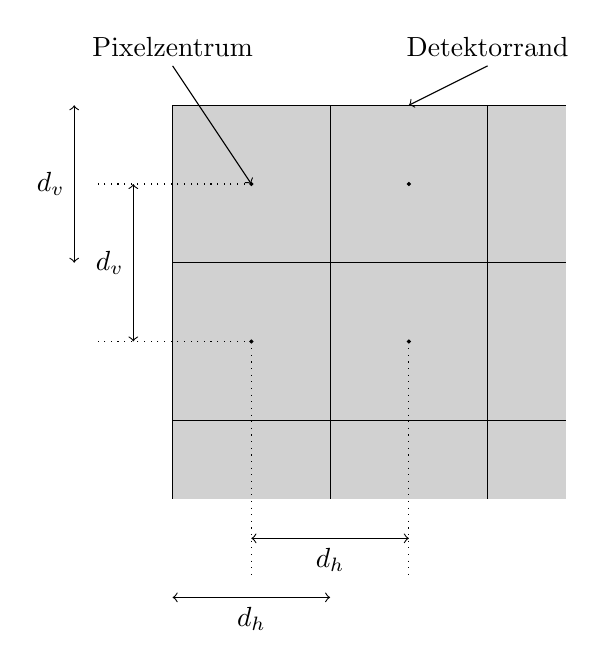
\begin{tikzpicture}
            \fill[black!60!white,opacity=0.3] (-2, 2) rectangle (3, -3);
            \draw (-2, 2) -- (2, 2) -- (2, -2) -- (-2, -2) -- (-2, 2);
            \draw (2, 2) -- (3, 2);
            \draw (-2, 0) -- (3, 0);
            \draw (0, 2) -- (0, -3);
            \draw (-2, 2) -- (-2, -3);
            \draw (2, -2) -- (2, -3);
            \draw (2, -2) -- (3, -2);
            \draw[fill=black] (-1, 1) circle (0.5pt);
            \draw[fill=black] (1, 1) circle (0.5pt);
            \draw[fill=black] (1, -1) circle (0.5pt);
            \draw[fill=black] (-1, -1) circle (0.5pt);

            % Verlängerungen
            \draw[dotted] (-1, 1) -- (-3, 1);
            \draw[dotted] (-1, -1) -- (-3, -1);
            \draw[dotted] (-1, -1) -- (-1, -4);
            \draw[dotted] (1, -1) -- (1, -4);

            % Pfeile und Beschriftungen
            \draw[->] (2, 2.5) -- (1, 2) node[pos=0, above] {Detektorrand};
            \draw[->] (-2, 2.5) -- (-1, 1) node[pos=0, above] {Pixelzentrum};
            \draw[<->] (-2.5, 1) -- (-2.5, -1) node[pos=0.5, left] {$d_v$};
            \draw[<->] (-3.25, 2) -- (-3.25, 0) node[pos=0.5, left] {$d_v$};
            \draw[<->] (-1, -3.5) -- (1, -3.5) node[pos=0.5, below] {$d_h$};
            \draw[<->] (-2, -4.25) -- (0, -4.25) node[pos=0.5, below] {$d_h$};
        \end{tikzpicture}
        \captionof{figure}{Pixelgeometrie}
        \label{fig:det_pixel}
    \end{minipage}
\end{figure}

\begin{figure}[!tb]
    \centering
    \begin{minipage}[b]{.5\textwidth}
        \centering
        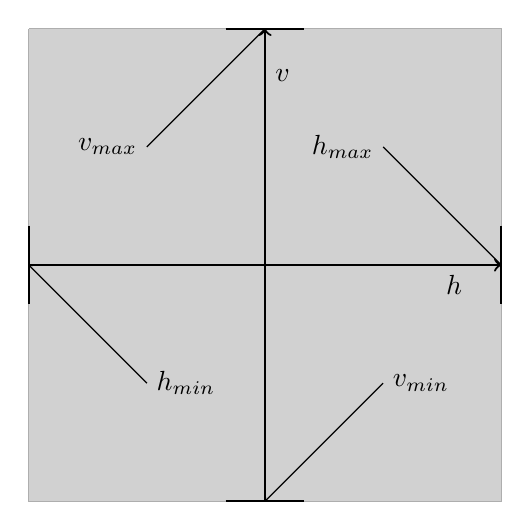
\begin{tikzpicture}[axis/.style={thick,->}]
            \draw[fill=black!60!white,opacity=0.3] (-3, 3) -- (3, 3) -- (3, -3) -- (-3, -3) -- (-3, 3);
            \draw[fill=black] (0,0) circle (0.5pt);

            % Achsen
            \draw[axis] (0, -3) -- (0, 3) node [pos=0.9, right] {$v$};
            \draw[axis] (-3, 0) -- (3, 0) node [pos=0.9, below] {$h$};

            % Markierungen
            \draw[thick] (-3, 0.5) -- (-3, -0.5);
            \draw[thick] (3, 0.5) -- (3, -0.5);
            \draw[thick] (-0.5, 3) -- (0.5, 3);
            \draw[thick] (-0.5, -3) -- (0.5, -3);

            % Beschriftungen
            \draw[->] (1.5, 1.5) -- (3, 0) node [pos=0, left] {$h_{max}$};
            \draw[->] (-1.5, -1.5) -- (-3, 0) node [pos=0, right] {$h_{min}$};
            \draw[->] (-1.5, 1.5) -- (0, 3) node [pos=0, left] {$v_{max}$};
            \draw[->] (1.5, -1.5) -- (0, -3) node [pos=0, right] {$v_{min}$};
        \end{tikzpicture}
        \caption{Detektorkoordinatensystem}
        \label{fig:det_koord}
    \end{minipage}%
    \begin{minipage}[b]{.5\textwidth}
        \centering
        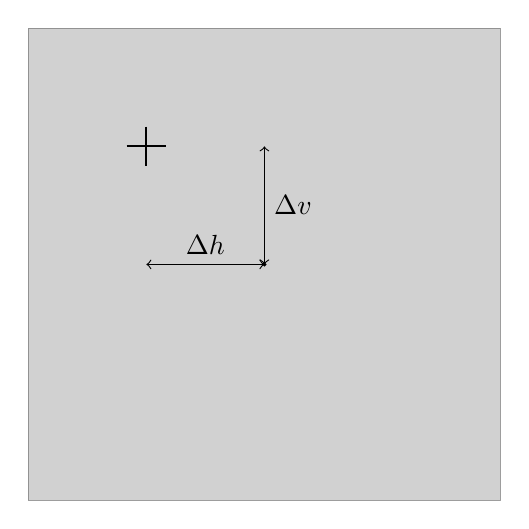
\begin{tikzpicture}
            \draw[fill=black!60!white,opacity=0.3] (-3, 3) -- (3, 3) -- (3, -3) -- (-3, -3) -- (-3, 3);
            \draw[fill=black] (0,0) circle (0.5pt);

            % Verschiebung
            \draw[thick] (-1.75, 1.5) -- (-1.25, 1.5);
            \draw[thick] (-1.5, 1.75) -- (-1.5, 1.25);

            % Pfeile & Beschriftung
            \draw[<->] (0, 1.5) -- (0, 0) node[pos=0.5,right] {$\Delta v$};
            \draw[<->] (0, 0) -- (-1.5, 0) node[pos=0.5,above] {$\Delta h$};
        \end{tikzpicture}
        \caption{Verschiebungsgeometrie}
        \label{fig:off_geometrie}
    \end{minipage}
\end{figure}

\subsubsection{Verschiebungen}

In einem idealen Modell sind die Strahlungsquelle und der Detektor genau aufeinander ausgerichtet, das heißt, dass der
Mittelpunkt der Strahlungsquelle und der Mittelpunkt des Detektors auf derselben Achse liegen. Durch den mechanischen
Aufbau einer realen Computertomographie-Anlage und deren händischer Justierung kommt es allerdings zu sowohl
einer horizontalen Verschiebung $\Delta h$ als auch einer vertikalen Verschiebung $\Delta v$ dieser Achse (siehe
Abbildung~\ref{fig:off_geometrie}). Von der Strahlungsquelle ausgehend trifft sie somit nicht mehr auf das Zentrum des
Detektors, sondern auf einen anderen Teil. Nimmt man Bezug auf die Detektorgeometrie, so müssen diese Verschiebungen
entsprechend berücksichtigt werden, da ansonsten ein verfälschtes Ergebnis berechnet wird. Dazu müssen die
Formeln~\ref{eq:det_h} und~\ref{eq:det_v} wie folgt umgeschrieben werden:

\begin{equation} 
    h_{min} + \frac{N_h \cdot d_h}{2} + \Delta h = 0
\end{equation}

\begin{equation}
    v_{min} + \frac{N_v \cdot d_v}{2}  + \Delta v = 0
\end{equation}

\subsubsection{Fehlende Projektionen}

Es leuchtet ein, dass Projektionen, die im Abstand von 180° aufgenommen wurden, das durchleuchtete Objekt
spiegelverkehrt darstellen. In der Theorie würde es also ausreichen, einen Halbkreis um das Objekt abzufahren, um alle
erforderlichen Informationen für die Rückprojektion zu gewinnen. In der Praxis kann es aufgrund mechanischer Fehler bei
der Rotation des Quelle-Detektor-Aufbaus allerdings dazu kommen, dass einzelne Projektionen übersprungen werden oder die
Winkelabstände zwischen zwei Projektionen verschieden groß sind. Das Abfahren eines Vollkreises dient dazu, die so
entstandenen Fehler durch Redundanzen zu minimieren.

\subsection{Geometrische Berechnungen}

\begin{itemize}
    \item Berechnung der Volumengeometrie
    \item Aufteilung in Teilvolumen
\end{itemize}

\subsection{Implementierung der Vorstufen}

\subsubsection{Wichtung}

Die Grundlage der Wichtungsoperation ist die in Abschnitt~\ref{sssec:fdk_wichtung} vorgestellte
Formel~\ref{eq:wichtung}:

\begin{equation*}
    w_{ij} = \frac{d_{det} - d_{src}}{\sqrt{(d_{det} - d_{src})^2 + h_j^2 + v_i^2}}
\end{equation*}

Es ist leicht zu sehen, dass sich der Wichtungsfaktor $w_{ij}$ zwar pro \gls{pixel} ändert, aber nicht von der konkreten
Projektion abhängig ist. Es ist daher möglich, die Berechnung der Wichtungsfaktoren am Anfang des Programms genau einmal
durchzuführen und in einer Wichtungsmatrix \texttt{m} zu speichern (siehe Quelltext~\ref{source:impl_gen_mat}). Die
Berechnung der Wichtungsmatrix hängt von mehreren geometrischen Parametern ab (vgl.\
Abschnitt~\ref{sssec:fdk_geometrie} und Abbildungen~\ref{fig:det_geometrie},~\ref{fig:det_pixel},~\ref{fig:det_koord},~\ref{fig:off_geometrie}):

\begin{itemize}
    \item \texttt{dim\_x}: Anzahl der \gls{pixel} in horizontaler Richtung. Entspricht der Anzahl der Detektorpixel in
          horizontaler Richtung $N_h$
    \item \texttt{dim\_y}: Anzahl der \gls{pixel} in vertikaler Richtung. Entspricht der Anzahl der Detektorpixel in
          vertikaler Richtung $N_v$
    \item \texttt{h\_min}: horizontaler Abstand vom Detektorrand zum Detektorzentrum in mm.
    \item \texttt{v\_min}: vertikaler Abstand vom Detektorrand zum Detektorzentrum in mm.
    \item \texttt{d\_sd}: Abstand von der Quelle zum Detektor. Entsprich der Differenz der Strecken $d_{det}$ (Abstand
          zwischen dem Objekt und dem Detektor) und $d_{src}$ (Abstand zwischen der Quelle und dem Objekt) bzw.\ der
          Summe ihrer Beträge:
          
          \begin{equation*}
              d_{det} - d_{src} = |d_{det}| + |d_{src}|
          \end{equation*}

    \item \texttt{l\_px\_row}: horizontale Länge eines \gls{pixel}s, also der horizontale Abstand zwischen den
          Mittelpunkten zweier aufeinanderfolgender \gls{pixel}. Entspricht der horizontalen Länge eines Detektorpixels
          $d_h$.
    \item \texttt{l\_px\_col}: vertikale Länge eines \gls{pixel}s, also der vertikale Abstand zwischen den
          Mittelpunkten zweier aufeinanderfolgender \gls{pixel}. Entspricht der vertikalen Länge eines Detektorpixels
          $d_v$.
\end{itemize}

\begin{code}
\begin{minted}[breaklines,breakafter=\,,fontsize=\small]{cuda}
__global__ void matrix_generation_kernel(float* m,
    std::uint32_t dim_x, std::uint32_t dim_y, std::size_t pitch,
    float h_min, float v_min, float d_sd, float l_px_row,
    float l_px_col)
{
    auto s = blockIdx.x * blockDim.x + threadIdx.x;
    auto t = blockIdx.y * blockDim.y + threadIdx.y;

    if((s < dim_x) && (t < dim_y))
    {
        auto row = reinterpret_cast<float*>(
            reinterpret_cast<char*>(m) + t * pitch);

        // Detektorkoordinaten in mm
        const auto h_s = (l_px_row / 2.f) + s * l_px_row + h_min;
        const auto v_t = (l_px_col / 2.f) + t * l_px_col + v_min;

        // berechne Wichtungsfaktor
        row[s] = d_sd * rsqrtf(d_sd * d_sd + h_s * h_s + v_t * v_t);
    }
}
\end{minted}
\captionof{listing}{Generierung der Wichtungsmatrix}
\label{source:impl_gen_mat}
\end{code}

Bei der Wichtung einer Projektion \texttt{p} kann der jeweilige Wichtungsfaktor aus der generierten Matrix \texttt{m}
ausgelesen und auf das zugehörige \gls{pixel} angewendet werden (siehe Quelltext~\ref{source:impl_weighting}). Die so
gewichtete Projektion wird dann im folgenden Schritt gefiltert.

\begin{code}
\begin{minted}[breaklines,breakafter=\,,escapeinside=||,fontsize=\small]{cuda}
__global__ void weighting_kernel(float* p, const float* m,
    std::uint32_t dim_x, std::uint32_t dim_y, std::size_t pitch,
    std::size_t m_pitch)
{
    auto s = blockIdx.x * blockDim.x + threadIdx.x;
    auto t = blockIdx.y * blockDim.y + threadIdx.y;

    if((s < dim_x) && (t < dim_y))
    {
        auto p_row = |\textbf{\textcolor{keyword-green}{reinterpret\_cast}}|<float*>(
            |\textbf{\textcolor{keyword-green}{reinterpret\_cast}}|<char*>(p) + t * pitch);
        auto m_row = |\textbf{\textcolor{keyword-green}{reinterpret\_cast}}|<const float*>(
            |\textbf{\textcolor{keyword-green}{reinterpret\_cast}}|<const char*>(m) + t * m_pitch);

        // Wichtung
        p_row[s] *= m_row[s];
    }
}
\end{minted}
\captionof{listing}{Wichtung einer Projektion}
\label{source:impl_weighting}
\end{code}

\subsubsection{Filterung}

Dem in Abschnitt~\ref{sssec:fdk_filter} vorgestellten Algorithmus entsprechend, folgt die Implementierung des
Filterschrittes dem nachstehenden Schema:

\begin{enumerate}
    \item einmalige Erzeugung und Fouriertransformation des Filters
    \item zeilenweise Fouriertransformation der Projektion
    \item Anwendung des Filters auf die jeweilige Projektionszeile im komplexen Raum
    \item inverse zeilenweise Fouriertransformation der Projektion
\end{enumerate}

Die Implementierung der Filtergenerierung entspricht der Formel~\ref{eq:filter_gen} und kann dem im Anhang befindlichen
Quelltext~\ref{app:filter_gen} entnommen werden. Dieser Filter wird dann zeilenweise auf jede Projektion angewendet.
Dazu werden der Filter und die einzelnen Projektionszeilen mit der \gls{cufft}-Bibliothek zunächst fouriertransformiert.
Im komplexen Raum werden dann die einzelnen Elemente der transformierten Projektionszeile mit den korrespondierenden
Elementen des transformierten Filters multipliziert (siehe Quelltext~\ref{source:impl_filter}). Ist dieser Vorgang
abgeschlossen, wird die Projektion wieder zurücktransformiert und normalisiert (siehe den angehängten
Quelltext~\ref{app:filter_norm}). Die Projektion ist dann bereit für die Rückprojektion.

\begin{code}
\begin{minted}[breaklines,breakafter=\,,fontsize=\small]{cuda}
__global__ void filter_application_kernel(
    cufftComplex* __restrict__ data,
    const cufftComplex* __restrict__ filter,
    std::uint32_t filter_size, std::uint32_t data_height,
    std::size_t pitch)
{
    auto x = blockIdx.x * blockDim.x + threadIdx.x;
    auto y = blockIdx.y * blockDim.y + threadIdx.y;

    if((x < filter_size) && (y < data_height))
    {
        auto row = reinterpret_cast<cufftComplex*>(
            reinterpret_cast<char*>(data) + y * pitch);

        row[x].x *= filter[x].x;
        row[x].y *= filter[x].y;
    }
}
\end{minted}
\captionof{listing}{Filterung einer Projektion}
\label{source:impl_filter}
\end{code}

\subsection{Implementierung der gefilterten Rückprojektion}

\begin{itemize}
    \item welche Konstanten und Variablen gibt es
    \item welche Schwierigkeiten können auftreten
\end{itemize}
